\documentclass[journal,12pt,twocolumn]{IEEEtran}

\usepackage{setspace}
\usepackage{gensymb}
\singlespacing
\usepackage[cmex10]{amsmath}
\usepackage{amssymb}
\usepackage{xurl}
\usepackage{tabularx}
\usepackage{amsthm}
\usepackage{comment}
\usepackage{mathrsfs}
\usepackage{txfonts}
\usepackage{stfloats}
\usepackage{bm}
\usepackage{cite}
\usepackage{cases}
\usepackage{subfig}
\usepackage{arydshln}
\usepackage{longtable}
\usepackage{multirow}

\usepackage{enumitem}
\usepackage{mathtools}
\usepackage{steinmetz}
\usepackage{tikz}
\usepackage{circuitikz}
\usepackage{verbatim}
\usepackage{tfrupee}
\usepackage[breaklinks=true]{hyperref}
\usepackage{graphicx}
\usepackage{tkz-euclide}
\usetikzlibrary{automata, positioning}
\usetikzlibrary{calc,math}
\usepackage{listings}
    \usepackage{color}                                            %%
    \usepackage{array}                                            %%
    \usepackage{longtable}                                        %%
    \usepackage{calc}                                             %%
    \usepackage{multirow}                                         %%
    \usepackage{hhline}                                           %%
    \usepackage{ifthen}                                           %%
    \usepackage{lscape}     
\usepackage{multicol}
\usepackage{chngcntr}
\usepackage{blkarray}

\DeclareMathOperator*{\Res}{Res}

\renewcommand\thesection{\arabic{section}}
\renewcommand\thesubsection{\thesection.\arabic{subsection}}
\renewcommand\thesubsubsection{\thesubsection.\arabic{subsubsection}}

\renewcommand\thesectiondis{\arabic{section}}
\renewcommand\thesubsectiondis{\thesectiondis.\arabic{subsection}}
\renewcommand\thesubsubsectiondis{\thesubsectiondis.\arabic{subsubsection}}


\hyphenation{op-tical net-works semi-conduc-tor}
\def\inputGnumericTable{}                                 %%

\lstset{
%language=C,
frame=single, 
breaklines=true,
columns=fullflexible
}
\begin{document}


\newtheorem{theorem}{Theorem}[section]
\newtheorem{problem}{Problem}
\newtheorem{proposition}{Proposition}[section]
\newtheorem{lemma}{Lemma}[section]
\newtheorem{corollary}[theorem]{Corollary}
\newtheorem{example}{Example}[section]
\newtheorem{definition}[problem]{Definition}

\newcommand{\BEQA}{\begin{eqnarray}}
\newcommand{\EEQA}{\end{eqnarray}}
\newcommand{\define}{\stackrel{\triangle}{=}}
\bibliographystyle{IEEEtran}
\raggedbottom
\setlength{\parindent}{0pt}
\providecommand{\mbf}{\mathbf}
\providecommand{\pr}[1]{\ensuremath{\Pr\left(#1\right)}}
\providecommand{\qfunc}[1]{\ensuremath{Q\left(#1\right)}}
\providecommand{\sbrak}[1]{\ensuremath{{}\left[#1\right]}}
\providecommand{\lsbrak}[1]{\ensuremath{{}\left[#1\right.}}
\providecommand{\rsbrak}[1]{\ensuremath{{}\left.#1\right]}}
\providecommand{\brak}[1]{\ensuremath{\left(#1\right)}}
\providecommand{\lbrak}[1]{\ensuremath{\left(#1\right.}}
\providecommand{\rbrak}[1]{\ensuremath{\left.#1\right)}}
\providecommand{\cbrak}[1]{\ensuremath{\left\{#1\right\}}}
\providecommand{\lcbrak}[1]{\ensuremath{\left\{#1\right.}}
\providecommand{\rcbrak}[1]{\ensuremath{\left.#1\right\}}}
\theoremstyle{remark}
\newtheorem{rem}{Remark}
\newcommand{\sgn}{\mathop{\mathrm{sgn}}}
\providecommand{\abs}[1]{\vert#1\vert}
\providecommand{\res}[1]{\Res\displaylimits_{#1}} 
\providecommand{\norm}[1]{\lVert#1\rVert}
%\providecommand{\norm}[1]{\lVert#1\rVert}
\providecommand{\mtx}[1]{\mathbf{#1}}
\providecommand{\mean}[1]{E[ #1 ]}
\providecommand{\fourier}{\overset{\mathcal{F}}{ \rightleftharpoons}}
%\providecommand{\hilbert}{\overset{\mathcal{H}}{ \rightleftharpoons}}
\providecommand{\system}{\overset{\mathcal{H}}{ \longleftrightarrow}}
	%\newcommand{\solution}[2]{\textbf{Solution:}{#1}}
\newcommand{\solution}{\noindent \textbf{Solution: }}
\newcommand{\cosec}{\,\text{cosec}\,}
\providecommand{\dec}[2]{\ensuremath{\overset{#1}{\underset{#2}{\gtrless}}}}
\newcommand{\myvec}[1]{\ensuremath{\begin{pmatrix}#1\end{pmatrix}}}
\newcommand{\mydet}[1]{\ensuremath{\begin{vmatrix}#1\end{vmatrix}}}
\newcommand*{\permcomb}[4][0mu]{{{}^{#3}\mkern#1#2_{#4}}}
\newcommand*{\perm}[1][-3mu]{\permcomb[#1]{P}}
\newcommand*{\comb}[1][-1mu]{\permcomb[#1]{C}}
\numberwithin{equation}{subsection}
\makeatletter
\@addtoreset{figure}{problem}
\makeatother
\let\StandardTheFigure\thefigure
\let\vec\mathbf
\renewcommand{\thefigure}{\theproblem}
\def\putbox#1#2#3{\makebox[0in][l]{\makebox[#1][l]{}\raisebox{\baselineskip}[0in][0in]{\raisebox{#2}[0in][0in]{#3}}}}
     \def\rightbox#1{\makebox[0in][r]{#1}}
     \def\centbox#1{\makebox[0in]{#1}}
     \def\topbox#1{\raisebox{-\baselineskip}[0in][0in]{#1}}
     \def\midbox#1{\raisebox{-0.5\baselineskip}[0in][0in]{#1}}
\vspace{3cm}
\title{AI1103 : Assignment 9}
\author{Yashas Tadikamalla - AI20BTECH11027}
\maketitle
\newpage
\bigskip
\renewcommand{\thefigure}{\arabic{figure}}
\renewcommand{\thetable}{\arabic{table}}
Download all python codes from 
\begin{lstlisting}
https://github.com/YashasTadikamalla/AI1103/tree/main/Assignment9/codes
\end{lstlisting}
%
and latex codes from 
%
\begin{lstlisting}
https://github.com/YashasTadikamalla/AI1103/blob/main/Assignment9/Assignment9.tex
\end{lstlisting}
\section*{CSIR-UGC NET-June 2013-Problem(72)}
Let $X_{1},X_{2},\dots$ be independent and identically distributed random variables each following a uniform distribution on (0,1). Denote $T_{n}=max\{ X_{1},X_{2},\dots,X_{n}\}$. Then, which of the following statements are true?
\begin{enumerate}
    \item $T_{n}$ converges to 1 in probability.
    \item $n(1-T_{n})$ converges in distribution.
    \item $n^{2}(1-T_{n})$ converges in distribution.
    \item $\sqrt{n}(1-T_{n})$ converges to 0 in probability.
\end{enumerate}
\section*{CSIR-UGC NET-June 2013-Solution(72)}
The PDF, CDF of each $X_{1},X_{2},X_{3},\dots$ is 
\begin{align}
\tag{72.1}
    f_{X_{i}}(x)=\begin{cases}
	1, & 0< x<1 \\~\\[-1em]
	0, & otherwise
	\end{cases} 
\end{align}
\begin{align}
\tag{72.2}
	F_{X_{i}}(x)=\begin{cases}
	x, & 0< x<1 \\~\\[-1em]
	1, & x\geq 1\\~\\[-1em]
	0, & otherwise
	\end{cases} 
\end{align}
$\forall i\in \mathbb{N}$.
Then, as $T_{n}=max\{ X_{1},X_{2},\dots,X_{n}\}$,
\begin{align}
\tag{72.3}
    f_{T_{n}}(x)=\begin{cases}
	nx^{n-1}, & 0< x<1 \\~\\[-1em]
	0, & otherwise
	\end{cases} \\
\tag{72.4}
	F_{T_{n}}(x)=\begin{cases}
	x^{n}, & 0< x<1 \\~\\[-1em]
	1, & x\geq 1\\~\\[-1em]
	0, & otherwise
	\end{cases} 
\end{align}
NOTE : If $Y=aX+b$, then
\begin{align}
\tag{72.5}
\label{eq:form}
    F_{Y}(y)=F_{X}\brak{\dfrac{y-b}{a}}
\end{align}
\begin{enumerate}
\item OPTION-1:\\
Convergence in Probability :\\
A sequence of random variables $X_{1},X_{2},X_{3},\dots$ converges in probability to a random variable $X$, shown by $X_{n}\xrightarrow[]{p}X$, if
\begin{align}
\tag{72.6}
    \displaystyle\lim_{n\to\infty}\pr{|X_{n}-X|\geq\epsilon}=0,\forall\epsilon>0
\end{align}
To evaluate : $\displaystyle\lim_{n\to\infty}\pr{|T_{n}-1|\geq\epsilon},\forall\epsilon>0$
\begin{align}
\tag{72.7}
    &\displaystyle\lim_{n\to\infty}\pr{|T_{n}-1|\geq\epsilon}=\displaystyle\lim_{n\to\infty}\pr{1-T_{n}\geq\epsilon}\\
\tag{72.8}
    &=\displaystyle\lim_{n\to\infty}\pr{T_{n}\leq1-\epsilon}=\displaystyle\lim_{n\to\infty}F_{T_{n}}(1-\epsilon)
\end{align}
\begin{align}
\tag{72.9}
    F_{T_{n}}(1-\epsilon)=\begin{cases}
	(1-\epsilon)^{n}, & 0< \epsilon<1 \\~\\[-1em]
	0, & \epsilon\geq 1
	\end{cases}
\end{align}
\begin{align}
\tag{72.10}
    \because\displaystyle\lim_{n\to\infty}(1-\epsilon)^{n}=0 \text{ for } 0< \epsilon<1\\
    \tag{72.11}
    \therefore \displaystyle\lim_{n\to\infty}\pr{|T_{n}-1|\geq\epsilon}=0,\forall\epsilon>0
\end{align}
$\therefore T_{n}$ converges to 1 in probability.
\item OPTION-2:\\
Convergence in Distribution :\\
A sequence of random variables $X_{1},X_{2},X_{3},\dots$ converges in distribution to a random variable $X$, shown by $X_{n}\xrightarrow[]{d}X$, if
\begin{align}
\tag{72.12}
    \displaystyle\lim_{n\to\infty}F_{X_{n}}(x)=F_{X}(x)
\end{align}
for all $x$ at which $F_{X}(x)$ is continuous.\\
To evaluate : $\displaystyle\lim_{n\to\infty}F_{n(1-T_{n})}(x)$\\ 
Substituting $a=-n,b=n$ in \eqref{eq:form},
\begin{align}
\tag{72.13}
    F_{n(1-T_{n})}(x)=F_{T_{n}}\brak{1-\dfrac{x}{n}}
\end{align}
\begin{align}
\tag{72.14}
    F_{T_{n}}\brak{1-\dfrac{x}{n}}=\begin{cases}
	\brak{1-\dfrac{x}{n}}^{n}, & 0< x<n \\~\\[-1em]
	1, & x\leq 0\\~\\[-1em]
	0, & x\geq n
	\end{cases} 
\end{align}
\begin{align}
\tag{72.15}
    \because\displaystyle\lim_{n\to\infty}\brak{1-\dfrac{y}{n}}^{n}=e^{-y}
\end{align}
\begin{align}
\tag{72.16}
\label{eq:cdf}
    \therefore\displaystyle\lim_{n\to\infty} F_{T_{n}}\brak{1-\dfrac{x}{n}}=\begin{cases}
	e^{-x}, & 0< x<n \\~\\[-1em]
	1, & x\leq 0\\~\\[-1em]
	0, & x\geq n
	\end{cases} 
\end{align}

\begin{center}
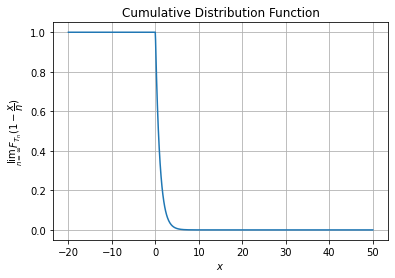
\includegraphics[scale=0.55]{Assignment9.png}
\end{center}

$\therefore n(1-T_{n})$ converges in distribution to a random variable with CDF in \eqref{eq:cdf}.
\item OPTION-3:\\
Convergence in Distribution :\\
A sequence of random variables $X_{1},X_{2},X_{3},\dots$ converges in distribution to a random variable $X$, shown by $X_{n}\xrightarrow[]{d}X$, if
\begin{align}
\tag{72.17}
    \displaystyle\lim_{n\to\infty}F_{X_{n}}(x)=F_{X}(x)
\end{align}
for all $x$ at which $F_{X}(x)$ is continuous.\\
To evaluate : $\displaystyle\lim_{n\to\infty}F_{n^{2}(1-T_{n})}(x)$\\ 
Substituting $a=-n^{2},b=n^{2}$ in \eqref{eq:form},
\begin{align}
\tag{72.18}
    F_{n^{2}(1-T_{n})}(x)=F_{T_{n}}\brak{1-\dfrac{x}{n^{2}}}
\end{align}
\begin{align}
\tag{72.19}
    F_{T_{n}}\brak{1-\dfrac{x}{n^{2}}}=\begin{cases}
	\brak{1-\dfrac{x}{n^{2}}}^{n}, & 0< x<n^{2} \\~\\[-1em]
	1, & x\leq 0\\~\\[-1em]
	0, & x\geq n^{2}
	\end{cases} 
\end{align}
\begin{align}
\tag{72.20}
    \because\displaystyle\lim_{n\to\infty}\brak{1-\dfrac{y}{n^{2}}}^{n}\text{ is not defined}
\end{align}
$\therefore n^{2}(1-T_{n})$ does not converge in distribution.
\item OPTION-4:\\
Convergence in Probability :\\
A sequence of random variables $X_{1},X_{2},X_{3},\dots$ converges in probability to a random variable $X$, shown by $X_{n}\xrightarrow[]{p}X$, if
\begin{align}
\tag{72.21}
    \displaystyle\lim_{n\to\infty}\pr{|X_{n}-X|\geq\epsilon}=0,\forall\epsilon>0
\end{align}
To evaluate :\\ $\displaystyle\lim_{n\to\infty}\pr{|\sqrt{n}(1-T_{n})-0|\geq\epsilon},\forall\epsilon>0$
\begin{align}
\tag{72.22}
    =\displaystyle\lim_{n\to\infty}\pr{1-T_{n}\geq\dfrac{\epsilon}{\sqrt{n}}}\\
\tag{72.23}
    =\displaystyle\lim_{n\to\infty}\pr{T_{n}\leq1-\dfrac{\epsilon}{\sqrt{n}}}\\
\tag{72.24}
    =\displaystyle\lim_{n\to\infty}F_{T_{n}}\brak{ 1-\dfrac{\epsilon}{\sqrt{n}}}
\end{align}
\begin{align}
\tag{72.25}
    F_{T_{n}}\brak{1-\dfrac{\epsilon}{\sqrt{n}}}=\begin{cases}
	\brak{1-\dfrac{\epsilon}{\sqrt{n}}}^{n}, & 0< \epsilon< \sqrt{n}\\~\\[-1em]
	0, & \epsilon\geq \sqrt{n}
	\end{cases}
\end{align}
\begin{align}
\tag{72.26}
    \because\displaystyle\lim_{n\to\infty}\brak{1-\dfrac{\epsilon}{\sqrt{n}}}^{n}=0 \text{ for } 0< \epsilon<\sqrt{n}\\
    \tag{72.27}
    \therefore \displaystyle\lim_{n\to\infty}\pr{|\sqrt{n}(1-T_{n})-0|\geq\epsilon}=0,\forall\epsilon>0
\end{align}
$\therefore\sqrt{n}(1-T_{n})$ converges to 0 in probability.
\end{enumerate}
\begin{lstlisting}
Hence, options 1), 2), 4) are correct.
\end{lstlisting}
\end{document}
